\documentclass[review]{elsarticle}

\usepackage{lineno,hyperref}
\modulolinenumbers[5]

\journal{Artificial Intelligence class at UFES}

%%%%%%%%%%%%%%%%%%%%%%%
%% Elsevier bibliography styles
%%%%%%%%%%%%%%%%%%%%%%%
%% To change the style, put a % in front of the second line of the current style and
%% remove the % from the second line of the style you would like to use.
%%%%%%%%%%%%%%%%%%%%%%%

%% Numbered
%\bibliographystyle{model1-num-names}

%% Numbered without titles
%\bibliographystyle{model1a-num-names}

%% Harvard
%\bibliographystyle{model2-names.bst}\biboptions{authoryear}

%% Vancouver numbered
%\usepackage{numcompress}\bibliographystyle{model3-num-names}

%% Vancouver name/year
%\usepackage{numcompress}\bibliographystyle{model4-names}\biboptions{authoryear}

%% APA style
%\bibliographystyle{model5-names}\biboptions{authoryear}

%% AMA style
%\usepackage{numcompress}\bibliographystyle{model6-num-names}

%% `Elsevier LaTeX' style
\bibliographystyle{elsarticle-num}
%%%%%%%%%%%%%%%%%%%%%%%

\let\mono\texttt% Change original \textit to now be equivalent to \texttt
\usepackage{cleveref}
\usepackage{listings}
\usepackage{xcolor}

\definecolor{codegreen}{rgb}{0,0.5,0}
\definecolor{codegray}{rgb}{0.5,0.5,0.5}
\definecolor{codepurple}{rgb}{0.58,0,0.82}
\definecolor{backcolour}{rgb}{0.95,0.95,0.95}

\lstdefinestyle{mystyle}{
    backgroundcolor=\color{backcolour},   
    commentstyle=\color{codegreen},
    keywordstyle=\color{magenta},
    numberstyle=\tiny\color{codegray},
    stringstyle=\color{codepurple},
    basicstyle=\ttfamily\footnotesize,
    captionpos=b,
    breaklines=true,
    breakatwhitespace=true,
    % numbers=left,e
    numbersep=5pt,
    tabsize=2,
    showtabs=true,
    showspaces=false,
}
\lstset{style=mystyle}

\begin{document}

\begin{frontmatter}

\title{Comparison of Machine Learning Algorithms for Classification of Hemophilia A Severity}

%% Group authors per affiliation:
\author{Henrique Coutinho Layber}
\address{Vitória, Espírito Santo, Brazil}

\begin{abstract}
This work compares the performance of different machine learning algorithms for the classification of a dataset of hemophilia A proteins. The algorithms used are: ZeroR, Naive-Bayes, Decision Tree, K-Nearest Neighbors, Multi-layer Perception, Random Forest, all present on \mono{scikit-learn}, and a custom-built algorithm called Heterogeneous Pooling. The best performer Random Forest with accuracy score of $0.65$.
\end{abstract}

\begin{keyword}
Machine learning\sep Hemophilia A\sep Classification
\end{keyword}

\end{frontmatter}

\linenumbers

\section{Introduction}

This work aims to compare the performance of different machine learning algorithms for the classification of a dataset of hemophilia A proteins. The algorithms used are: ZeroR (ZR), Naive-Bayes (NB), Decision Tree (DT), K-Nearest Neighbors (KNN), Multi-layer Perception (MLP), Random Forest (RF), all present on \mono{scikit-learn}, and a custom-built algorithm called Heterogeneous Pooling (HP).

\section{Database}

\subsection{Domain Description}

Hemophilia A is a genetic disorder that impairs the blood's ability to clot. It is caused by the deficiency of clotting factor VIII (FVIII) and it's the most common hemophilia type. 
It's severity is classified into three categories: mild, moderate, and severe. The classification is based on the amount of FVIII present in the blood where the severity increases as the amount of FVIII decreases.

The dataset describe point mutations on the FVIII protein. They describe the position of the mutation and the amino acids before and after the mutation.

\subsection{Definition of Classes and Features}

Classes are the severity of the disease, which can be mild, moderate, or severe. As per the complimentary description paper excerpt\cite{paperexcerpt}, features other than the target class are 18 data points that describe some characteristics of the FVIII protein, distributed in:
\begin{itemize}
    \item Genetic characteristics: \mono{AA\_HGVS}, \mono{AA\_Legacy}, \mono{aa1}, \mono{A\_dist}

    \item Structural characteristics at the mutation site: \mono{phi}, \mono{psi}, \mono{phi}, \mono{bfactor}, \mono{areaSAS}, \mono{areaSES}, \mono{kdHydrophobicity}, \mono{ConsurfDB}

    \item Characteristics of the interaction network of residues at the mutation site: \mono{degree}, \mono{betweenness}, \mono{closeness}, \mono{burts}, \mono{pr}, \mono{auth}, \mono{kcore}
\end{itemize}

Out of those, only \mono{aa1} and \mono{aa2} are categorical, the rest are numerical.
The exact meaning of each feature is abstracted by the professor that provided the dataset, affirming that all of those are relevant to the classification task, so the feature selection step is skipped.

\subsection{Number of Instances} \label{instances}

The dataset comprises 415 instances of point mutations in the FVIII protein, all totally populated (no missing values). This makes any instance removal unnecessary. There are $192$ Mild, $152$ Severe, and $71$ Moderate instances.

\section{The Heterogeneous Pooling Method}

The Heterogeneous Pooling (HP) is a hybrid prediction model, being an ensemble on multiples sets of $3$ models each. The hyperparameter $n$ is the number of sets of models.

In the training process, the first set of models are trained with all $X_{col}$ columns of the dataset $X$. Every subsequent sets are trained with a random number $d, d \in [2,X_{col})$ of columns removed from the dataset. The columns to be removed are chosen with a probability proportional to the \emph{ANOVA F-value} of each column. It is relevant to note that for each column removed, the  \emph{ANOVA F-value} for the remaining columns should be recalculated, since variances (which \emph{ANOVA F-value} is based on) will be affected by the absence of the column.

On the prediction process, the model will predict the class of each instance with each model, and then the most frequent class will be chosen. In case of a tie, any class with the highest occurrence in the original dataset will be chosen.

On \cref{lst:hp}, the implementation of the HP algorithm is shown. In the implementation, the class \lstinline{Label} is a single set of $3$ models, in a way that remembers the columns removed during training, to remove the same columns for prediction. The full implementation can be found on \href{https://github.com/Henriquelay/AI-classes/blob/main/Trab1/Trab1_Henrique_Layber.ipynb}{GitHub}.

\section{Description of the Experiments Performed and their Results}

The models were trained with a $10$-fold cross-validation, with the dataset being shuffled before each fold (\mono{RepeatedStratifiedKFold}).
% A pipeline was used to scale the dataset with \mono{scikit-learn}'s \mono{StandardScaler} and then train the models. This gives the advantage to scale the dataset of the fold, instead of the whole dataset at once, which is a more realistic test scenario (since we don't use the knowledge of a datum we haven't seen yet), and increasing precision in some models. Models with hyperparameters were optimized with \mono{GridSearchCV}, using 4 folds.

% \Cref{fig:acc_pipe_comp} shows the comparison of the models with and without the pipeline, models without pipeline are post-fixed with \mono{NP}. 
\Cref{fig:models_comp} shows for the comparison between the different models. The mean and standard deviation of the models are shown on \cref{tab:mean_std}. \Cref{tab:p_values} holds the p-values of the models.

% \begin{figure}[h]
%     \centering
%     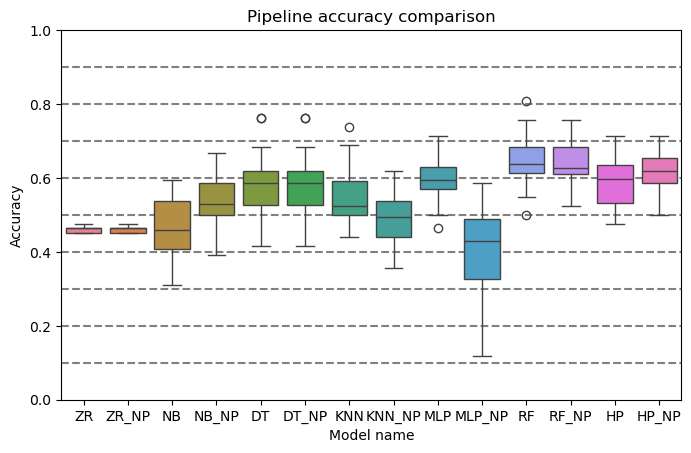
\includegraphics[width=0.9\textwidth]{pipeline_comparison.png}
%     \caption{Accuracy of the models with vs without the pipeline}
%     \label{fig:acc_pipe_comp}
% \end{figure}

\begin{figure}[h]
    \centering
    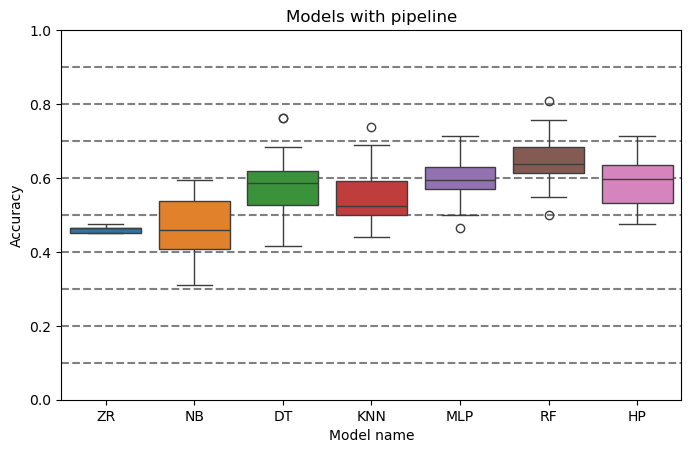
\includegraphics[width=0.9\textwidth]{comparison_with_pipeline.png}
    \caption{Accuracy of the models with pipelines}
    \label{fig:models_comp}
\end{figure}

\begin{table}[h]
    \centering
    \begin{tabular}{|c|c|c|c|c|}
        \hline
        Model & Mean & StDev. & Lower Limit & Upper Limit \\
        \hline
        ZR & 0.46 & 0.01 & 0.46 & 0.47 \\
        NB & 0.46 & 0.08 & 0.43 & 0.49 \\
        DT & 0.58 & 0.08 & 0.55 & 0.61 \\
        KNN & 0.55 & 0.07 & 0.53 & 0.58 \\
        MLP & 0.60 & 0.06 & 0.57 & 0.62 \\
        RF & 0.65 & 0.06 & 0.63 & 0.67 \\
        HP & 0.59 & 0.06 & 0.57 & 0.62 \\
        \hline
    \end{tabular}
    \caption{Mean and standard deviation of the models}
    \label{tab:mean_std}
\end{table}

% ZR	0.927	**0.000**	**0.000**	**0.000**	**0.000**	**0.000**
% 0.962	NB	**0.000**	**0.000**	**0.000**	**0.000**	**0.000**
% **0.000**	**0.000**	DT	**0.046**	0.354	**0.000**	0.381
% **0.000**	**0.000**	0.131	KNN	**0.000**	**0.000**	**0.004**
% **0.000**	**0.000**	0.451	**0.007**	MLP	**0.000**	0.819
% **0.000**	**0.000**	**0.002**	**0.000**	**0.002**	RF	**0.000**
% **0.000**	**0.000**	0.543	**0.028**	0.866	**0.004**	HP

\begin{table}[h]
    \centering
    \begin{tabular}{|c|c|c|c|c|c|c|}
        \hline
        ZR & 0.927 & \textbf{0.000} & \textbf{0.000} & \textbf{0.000} & \textbf{0.000} & \textbf{0.000} \\
        0.962 & NB & \textbf{0.000} & \textbf{0.000} & \textbf{0.000} & \textbf{0.000} & \textbf{0.000} \\
        \textbf{0.000} & \textbf{0.000} & DT & \textbf{0.046} & 0.354 & \textbf{0.000} & 0.381 \\
        \textbf{0.000} & \textbf{0.000} & 0.131 & KNN & \textbf{0.000} & \textbf{0.000} & \textbf{0.004} \\
        \textbf{0.000} & \textbf{0.000} & 0.451 & \textbf{0.007} & MLP & \textbf{0.000} & 0.819 \\
        \textbf{0.000} & \textbf{0.000} & \textbf{0.002} & \textbf{0.000} & \textbf{0.002} & RF & \textbf{0.000} \\
        \textbf{0.000} & \textbf{0.000} & 0.543 & \textbf{0.028} & 0.866 & \textbf{0.004} & HP \\
        \hline
    \end{tabular}
    \caption{Wilcoxon (lower triangle) and corrected dependent t-test (upper triangle) p-values of the models (main diagonal)}
    \label{tab:p_values}
\end{table}


\section{Conclusions}

HP is a good model, being statistically similar to some of the best models, and having a good accuracy. 
It performed as well as the other \emph{GridSearch} optimized models, only having a single hyperparameter to tune.
However, it is ill-advised to use it in a real scenario, it is way harder to debug and maintain, and it's performance is not guaranteed to be the same in a different dataset, for not as much benefit. Moreover, it's training process is very slow, since it trains multiple models multiple times.

The worst models are ZR and NB, with accuracies of $0.46$. The best model is RF, with an accuracy of $0.65$. HP offers a good trade-off between performance and complexity, with an accuracy of $0.59$ due to only having a single hyperparameter.


\subsection{General Analysis of the Results}

Three models are not statistically different from eachother: DT, MLP and HP. They are also very similar in performance, reaching high accuracy of $0.58$, $0.60$ and $0.59$ respectively. This is because HP is a hybrid model that uses DT as it's main (most accurate when alone) estimator. It's similarity with MLP strikes due to the inner workings of the HP model: it funcions just like a perceptron. It receives data from NB, DT and KNN and the most represented prediction is replicated, much like a perception with equal weights. The other less accurate models get outvoted by the two other more accurate models.

Bringing attention to some outliers on the hypothesis tests, some pairs (MLP and RF, ZR and NB) showed a very high p-value on the Dependant T-test, but a very low Wilcoxon test. This is due to the Dependant T-test being more sensitive to outliers, and the Wilcoxon test being more reliable when the dataset is unbalanced (\cref{instances}). And smaller outliers occur on the other models, but they are not as significant as the ones mentioned.

\subsection{Contributions of the Work}

The main contribution of this work is the comparison of HP model, which uses multiple sets of models to predict the class of a sample via voting.

\subsection{Improvements and Future Work}

The HP model could be improved by using a more sophisticated method to choose the columns to be removed, and by using a more sophisticated method to choose the best model to predict the class of a sample.

\appendix

\section{Heterogeneous Pooling Implementation} \label{lst:hp}

\begin{lstlisting}[
    language=Python,
    caption={Heterogeneous Pooling Algorithm},
]
def pick_columns(self, X: np.ndarray, y, n_columns: int) -> list[int]:
    """Select the `n_columns` to be removed from the dataset, with weight proportional to ANOVA F-value."""
    removed_cols = []
    current_cols = list(range(X.shape[1]))
    dataset = X.copy()
    # Need to recalculate the weights every time a column is removed
    for _ in range(n_columns):
        weigths, _ = anova_f(dataset, y)
        weigths /= weigths.sum()
        while True:
            picked_col = int(self.rng.choice(current_cols, p=weigths))
            removed_cols.append(picked_col)
            dataset = np.delete(dataset, current_cols.index(picked_col), axis=1)
            current_cols.remove(picked_col)
            break

    return removed_cols

def fit(self, X: pd.DataFrame, y: pd.Series):
    self.layers = [Layer() for _ in range(self.n_samples)]
    X, y = check_X_y(X, y)

    # Saves the majority class to be used in case of a tie
    counter = Counter(y)
    self.majority = max(counter, key=counter.get)
    self.counter = counter

    # The first estimators are trained on the original dataset
    self.layers[0].fit(X, y, [])

    # The remaining are trained on the dataset with at least 2 columns removed, repeated
    for layer in self.layers[1:]:
        n_features = X.shape[1]
        n_features_to_drop = self.rng.randint(2, n_features - 1)
        features_to_drop = self.pick_columns(X, y, n_features_to_drop)
        layer.fit(X, y, features_to_drop)

def determine_output(self, predictions: Iterable[int]) -> int:
    """Returns the most frequent if there is a tie, otherwise the most common value."""
    counter = Counter(predictions)
    max_count = counter.most_common(1)[0][1]
    max_count_elements = [k for k, v in counter.items() if v == max_count]
    if len(max_count_elements) > 1:
        for k, _ in self.counter.most_common():
            if k in max_count_elements:
                return k
    return max_count_elements[0]

def predict(self, X: pd.DataFrame):
    # A list of layers, each layer containing a list of models, each model containing a list of predictions for X
    predictions_per_layer: list[list[np.array]] = [
        layer.predict(X) for layer in self.layers
    ]
    # A list of predictions for each class, each containing the predictions of all layers and models
    predictions_per_class: list[np.array] = [
        [
            model_predictions[i]
            for layer in predictions_per_layer
            for model_predictions in layer
        ]
        for i in range(X.shape[0])  # For each sample
    ]
    result = [
        self.determine_output(predictions) for predictions in predictions_per_class
    ]
    return pd.DataFrame(result)
\end{lstlisting}

% \bibliography{mybibfile}

\end{document}
